\begin{center}
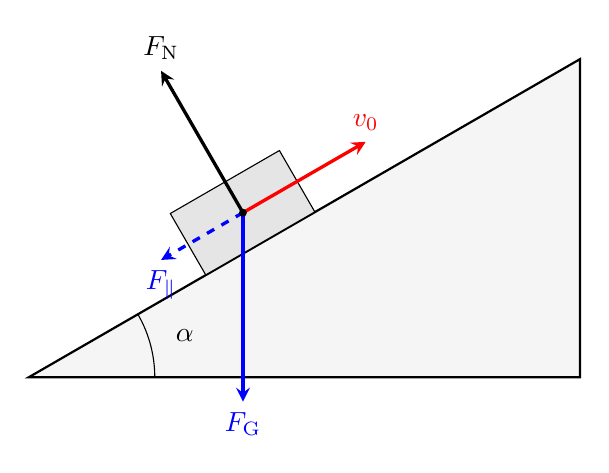
\begin{tikzpicture}[>=stealth]
 \draw[thick, fill=gray!8] (0,0) -- (7.00,0) -- (7.00,4.04) -- cycle;
 \draw (1.6,0) arc (0:30:1.6);
 \node at (1.98,0.53) {$\alpha$};
 \begin{scope}[shift={(2.94,1.70)}, rotate=30]
  \draw[fill=gray!20] (-0.8,0) rectangle (0.8,0.9);
 \end{scope}
 \draw[->, very thick, blue] (2.72,2.09) -- ++(-90.00:2.40) node[anchor=north] {$F_\mathrm{G}$};
 \draw[->, very thick, black] (2.72,2.09) -- ++(120.00:2.08) node[anchor=south] {$F_\mathrm{N}$};
 \draw[->, very thick, red] (2.72,2.09) -- ++(30.00:1.80) node[anchor=south] {$v_0$};
 \draw[->, very thick, blue, dashed] (2.72,2.09) -- ++(210.00:1.20) node[anchor=north] {$F_\parallel$};
 \fill (2.72,2.09) circle (0.05);
\end{tikzpicture}
\end{center}

Normalkraft und Komponente der Gewichtskraft senkrecht zur Ebene heben sich auf. Die resultierende Kraft ist die Hangabtriebskraft $F_\parallel = m\,g\sin\alpha$, die den Körper abwärts beschleunigt. Er wird also gleichmässig verzögert mit
\begin{align}
 a &= \frac{F_\parallel}{m} = \aHaF = \gE\cdot\sin\left(\wiO\right) = \aHa
\end{align}
Er kehrt um, wenn seine Geschwindigkeit null geworden ist, also nach
\begin{align}
 t &= \frac{v_0}{a} = \tUmF \\
   &= \frac{\vAn}{\gE\cdot\sin\left(\wiO\right)} \\
   &= \tUm \approx \result{\tUmP{0}{2}}
\end{align}
